\documentclass[border=6pt]{standalone}
\usepackage{amsmath}
\usepackage{amssymb}
\usepackage{tikz}
\usepackage{xcolor}
\usetikzlibrary{arrows.meta,calc,positioning,shapes.geometric}
\begin{document}
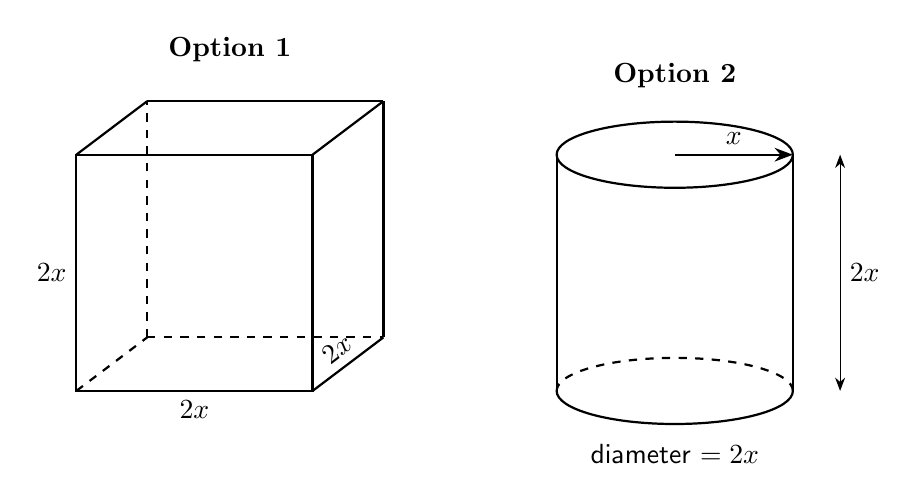
\begin{tikzpicture}[font=\sffamily]
  % ---------- Option 1: rectangular prism, square base, every edge = 2x ----------
  \def\side{3.0}
  \coordinate (dx1) at (0.9,0.68);

  \coordinate (fbl) at (0,0);
  \coordinate (fbr) at (\side,0);
  \coordinate (ftr) at (\side,\side);
  \coordinate (ftl) at (0,\side);
  \coordinate (bbl) at ($(fbl)+(dx1)$);
  \coordinate (bbr) at ($(fbr)+(dx1)$);
  \coordinate (btr) at ($(ftr)+(dx1)$);
  \coordinate (btl) at ($(ftl)+(dx1)$);

  \draw[thick] (fbl) -- (fbr) -- (ftr) -- (ftl) -- cycle;
  \draw[thick, dashed] (bbl) -- (bbr);
  \draw[thick, dashed] (bbl) -- (btl);
  \draw[thick] (bbr) -- (btr);
  \draw[thick] (btl) -- (btr);
  \draw[thick, dashed] (fbl) -- (bbl);
  \draw[thick] (fbr) -- (bbr);
  \draw[thick] (ftl) -- (btl);
  \draw[thick] (ftr) -- (btr);

  \node[font=\bfseries] at ($(ftl)!0.5!(btr)+(0,1.0)$) {Option 1};
  \node[below] at ($(fbl)!0.5!(fbr)$) {$2x$};
  \node[left] at ($(fbl)!0.5!(ftl)$) {$2x$};
  \path (fbr) -- (bbr) node[midway, sloped, above] {$2x$};

  % ---------- Option 2: cylinder, radius x, height 2x (diameter 2x = prism base side) ----------
  \def\R{1.5}
  \def\Ry{0.42}
  \def\H{3.0}
  \coordinate (cyl) at (7.6,0);

  % bottom ellipse: far/upper half hidden (dashed), near/lower half visible (solid)
  \draw[thick, dashed] ($(cyl)+(\R,0)$) arc (0:180:1.5 and 0.42);
  \draw[thick] ($(cyl)+(-\R,0)$) arc (180:360:1.5 and 0.42);

  % top ellipse: fully visible
  \draw[thick] ($(cyl)+(0,\H)$) ellipse (1.5 and 0.42);

  % side tangent lines
  \draw[thick] ($(cyl)+(-\R,0)$) -- ($(cyl)+(-\R,\H)$);
  \draw[thick] ($(cyl)+(\R,0)$)  -- ($(cyl)+(\R,\H)$);

  \node[font=\bfseries] at ($(cyl)+(0,\H+1.0)$) {Option 2};

  % radius label on the visible top ellipse
  \draw[-Stealth, thick] ($(cyl)+(0,\H)$) -- ($(cyl)+(\R,\H)$);
  \node[above] at ($(cyl)+(\R/2,\H)$) {$x$};

  % height label
  \draw[Stealth-Stealth] ($(cyl)+(\R+0.6,0)$) -- ($(cyl)+(\R+0.6,\H)$);
  \node[right] at ($(cyl)+(\R+0.6,\H/2)$) {$2x$};

  % diameter label along the base
  \node[below] at ($(cyl)+(0,-0.55)$) {diameter $=2x$};
\end{tikzpicture}
\end{document}
